\documentclass[11pt,a4paper]{article}

\usepackage[utf8]{inputenc}
\usepackage[T1]{fontenc}
\usepackage[spanish,es-noquoting,es-tabla,es-nodecimaldot]{babel}
\usepackage{lmodern}
\usepackage{microtype}
\usepackage[a4paper,margin=2.3cm]{geometry}
\usepackage{graphicx}
\usepackage{booktabs}
\usepackage{tabularx}
\usepackage{array}
\usepackage{caption}
\usepackage{subcaption}
\usepackage{float}
\usepackage{enumitem}
\usepackage[dvipsnames]{xcolor}
\usepackage[hidelinks]{hyperref}

\graphicspath{{../outputs/figuras/}}
\captionsetup{font=small,labelfont=bf}
\setlist{itemsep=2pt,topsep=4pt}
\setlength{\parskip}{4pt}
\renewcommand{\arraystretch}{1.15}
\newcolumntype{L}{>{\raggedright\arraybackslash}X}
\newcommand{\var}[1]{\texttt{\small #1}}

\title{\textbf{Clustering the Star}\\[4pt]
\large Segmentación de clientes de Mercedes-Benz}
\author{Equipo \textbf{Benji}\\[2pt]
Víctor Tirado · Alfonso del Álamo · Vicente Díaz\\[6pt]
\small III Malackathon 2026 · Reto Mercedes-Benz Group Services Madrid}
\date{Octubre de 2026}

\begin{document}
\maketitle

\section{Qué hemos hecho y cómo leer este informe}

El reto consiste en segmentar a los clientes de Mercedes-Benz con K-Means y describir cada segmento de forma que un equipo de marketing lo pueda usar: qué ofrecerle, cómo cuidar su mantenimiento, cómo fidelizarlo y cómo hablarle.

Trabajamos con 302.850 filas de clientes de Suiza (66\,\%) y Austria (34\,\%). Cada reto básico tiene su notebook, y aquí contamos lo que hicimos en cada uno: la decisión que tomamos, el dato que la respalda y lo que salió. Los notebooks están ejecutados y documentados, por si alguien quiere ver el detalle.

\begin{center}
\small
\begin{tabularx}{\linewidth}{l>{\raggedright\arraybackslash}p{5.2cm}L}
\toprule
Reto & Notebook & Qué contiene \\
\midrule
1 · EDA y calidad & \var{01\_eda\_calidad} & Exploración, nulos, inconsistencias y columnas descartadas \\
2 · Features & \var{02a\_features\_cliente}, \var{02b\_pipeline} & Tabla por cliente, variables derivadas y pipeline \\
3 · K-Means & \var{03\_kmeans} & Elección de variables y de $k$, modelo final \\
4 · Interpretación & \var{04\_interpretacion} & Perfil, nombre y plan de cada segmento, y dashboard \\
\bottomrule
\end{tabularx}
\end{center}

Toda la lógica está en \var{src/} y los notebooks la llaman, así que los tres trabajamos siempre sobre los mismos datos. Usamos semilla fija (42) en todo lo que tiene azar, para que los resultados se puedan repetir.

\section{Reto 1 · Exploración y calidad de los datos}

\subsection*{Lo primero: ¿qué es una fila?}

Lo que más condicionó todo el trabajo lo vimos nada más empezar: el CSV no tiene una fila por cliente, sino una por cada \textbf{relación cliente-vehículo}. Las 302.850 filas corresponden a 173.456 clientes y 244.519 vehículos. Al comprobar qué columnas cambian dentro de un mismo cliente salen tres niveles:

\begin{itemize}
  \item \textbf{Del cliente} (idénticas en todas sus filas): edad, género, país, antigüedad, financiación, consentimientos y datos de su código postal.
  \item \textbf{Del vehículo}: modelo, clase, motor y fecha de matriculación.
  \item \textbf{De la relación}: rol, si el vehículo está activo, visitas al taller y telemetría.
\end{itemize}

El 73\,\% de los clientes tiene un solo coche, pero el 27\,\% que tiene varios acumula el \textbf{58\,\% de las filas}, y 908 cuentas con 20 o más vehículos (el 0,5\,\% de los clientes) se llevan el 16\,\%. Si agrupáramos filas, un cliente con 11 coches contaría 11 veces y podría acabar en varios segmentos a la vez. Por eso decidimos \textbf{segmentar a nivel cliente} y resumir sus vehículos. Esa tabla se construye en el reto 2.

\subsection*{Nulos: cuatro bloques, cuatro causas}

\begin{table}[H]
\centering\small
\begin{tabularx}{\linewidth}{>{\raggedright\arraybackslash}p{3.6cm}cLL}
\toprule
Columnas & Nulos & Causa & Qué hacemos \\
\midrule
Telemetría (distancia, velocidad, consumo, horas) & 57--61\,\% & Estructural: no hay coche conectado. El 40\,\% de los clientes no tiene ningún dato & Fuera del modelo base y un flag \var{has\_telemetry}. Lo comprobamos en el reto 3 \\
\var{engine\_concept} / \var{fuel\_type} & 44\,\% / 59\,\% & Hueco de registro: no depende del año del coche & Rellenamos el motor a partir de la versión comercial (reto 2). Fuera \var{fuel\_type}, que repite el motor \\
Poder adquisitivo y población & 6\,\% & Código postal ausente o sin datos & Mediana \textbf{de su país}: Suiza (51.000\,€) y Austria (30.000\,€) no se parecen \\
\var{gender\_derived} & 11\,\% & Es un dato inferido, no declarado & Fuera del modelo: no queremos segmentar por un dato sensible inferido \\
\bottomrule
\end{tabularx}
\end{table}

\subsection*{Inconsistencias que encontramos}

\begin{itemize}
  \item \textbf{Un pico de antigüedad en 36 meses}: 21.179 clientes (12\,\%) tienen exactamente 36 meses, unas 9 veces más que los meses vecinos, y con coches más viejos que la media. Tiene toda la pinta de ser un valor por defecto de carga, así que lo marcamos con un flag (\var{tenure\_is\_default}).
  \item \textbf{Columnas que dicen lo mismo}: \var{role\_type} = B2B es exactamente \var{role} = DRIVER; \var{currently\_connected\_vehicles} coincide con el número de vehículos activos salvo en 4 clientes; y las cinco variables socioeconómicas se reducen a dos (correlaciones de 0,96 a 1,00). Nos quedamos con una de cada.
  \item \textbf{Columnas inservibles}: las \var{*\_mode} son texto y a veces traen listas enteras de valores; los contadores de telemetría llegan a 1.450 millones. Fuera.
  \item \textbf{Valores extremos} poco creíbles (velocidades medias de más de 150\,km/h, consumos de 50\,l/100\,km): los recortamos en el pipeline.
\end{itemize}

Descartamos también los identificadores (\var{client\_id}, \var{vehicle\_id}, \var{zipcode}) y las columnas con demasiado detalle (\var{vehicle\_type}, con 1.436 valores, y \var{model\_series}).

\subsection*{Cómo son los clientes}

Contados por cliente y no por fila: la base es madura (el 61\,\% tiene 45 años o más), el 73\,\% solo ha tenido un coche, mandan los SUV y las clases C y A, y hay un bloque importante de furgonetas. El 23\,\% tiene algún eléctrico o enchufable, y esa proporción \textbf{crece con la edad} (del 12\,\% en menores de 25 años al 28\,\% entre 55 y 64), más en Austria (31\,\%) que en Suiza (20\,\%). El 26\,\% tiene un leasing activo, el 10\,\% no tiene ningún coche activo y casi todos aceptan el email como canal (98\,\%).

\begin{figure}[H]
\centering
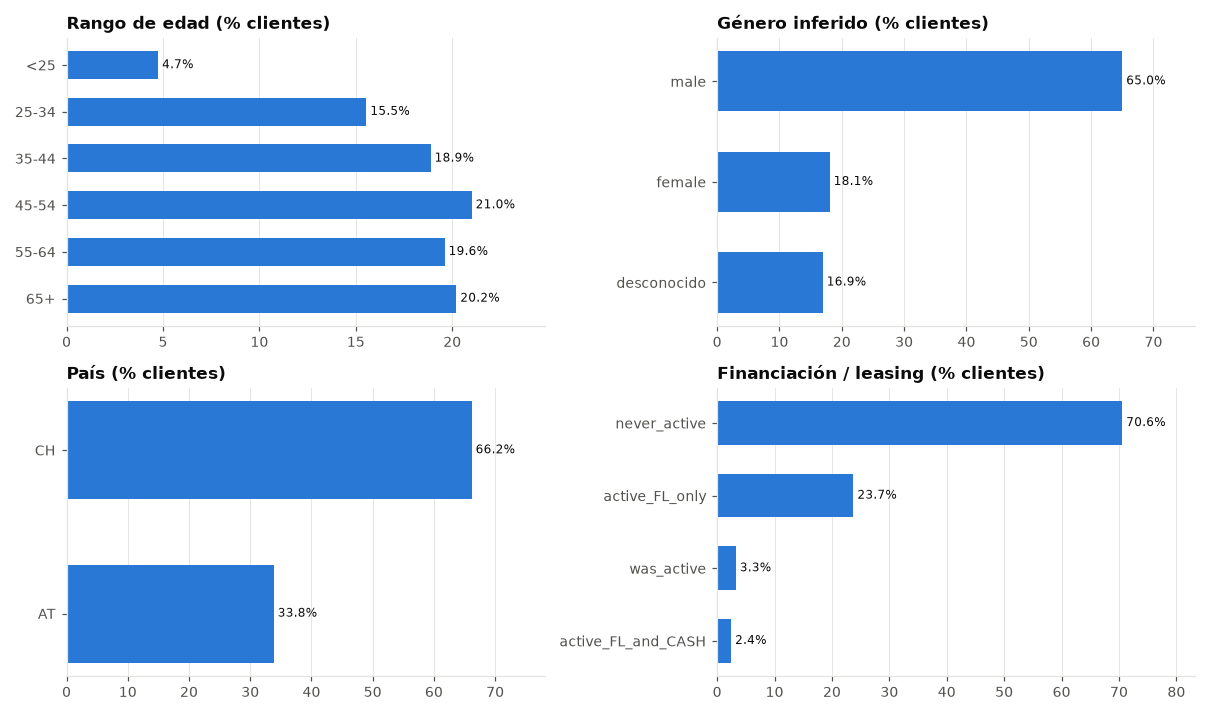
\includegraphics[width=0.82\linewidth]{01_demografia.png}
\caption{Edad, género inferido, país y situación de leasing, contados por cliente.}
\end{figure}

\section{Reto 2 · Feature engineering}

\subsection*{De filas a clientes}

Las columnas del cliente las tomamos tal cual. Las del vehículo hay que resumirlas, y aquí tomamos dos decisiones:

\begin{itemize}
  \item Para lo que no se puede promediar (la clase o el motor) elegimos un \textbf{vehículo principal}: el actual matriculado más recientemente o, si no tiene ninguno actual, el más reciente.
  \item Para el resto usamos resúmenes de todos sus coches: cuántos tiene, la media de visitas en garantía o la proporción de enchufables.
\end{itemize}

\textbf{Motor.} En el reto 1 vimos que la versión comercial (``GLC 300 e'', ``C 220 d''...) casi siempre delata el motor. El EDA daba una pureza del 99\,\%, pero esa cifra es la media por versión; ponderada por filas es el 95,5\,\%, porque hay versiones ambiguas (la ``C 220 d'' ha sido combustión o mild hybrid según la generación). Por eso solo usamos las versiones con al menos un 90\,\% de pureza y 5 casos conocidos. Además, la familia EQ es siempre eléctrica. Con eso, el motor desconocido del vehículo principal baja del 40\,\% al 18\,\%.

\subsection*{Variables derivadas}

\begin{table}[H]
\centering\small
\begin{tabularx}{\linewidth}{>{\raggedright\arraybackslash}p{4.1cm}L}
\toprule
Variable & De dónde sale y por qué \\
\midrule
\var{main\_vehicle\_age} & Años desde la matriculación del vehículo principal (referencia: 15/10/2026). Mide lo cerca que está la renovación, la base de las ofertas de coche nuevo \\
\var{n\_vehicles} & Número de vehículos del cliente. Separa a particulares de flotas \\
\var{share\_plugin\_ev} & Proporción de eléctricos o enchufables entre sus coches con motor conocido. Afinidad con la electrificación \\
\var{workshop\_visits\_mean} & Visitas al taller \textbf{en garantía} por vehículo. Promediamos para no premiar a quien simplemente tiene más coches \\
\var{tenure\_is\_default} & 1 si su antigüedad es el 36 por defecto, para que el modelo no lo tome como dato real \\
\var{ppi\_rel} & Poder adquisitivo de su zona dividido entre la mediana de su país (ver abajo) \\
\var{main\_class\_group} & Las 42 clases de modelo agrupadas en 7 segmentos de mercado (compacto, medio, ejecutivo...) \\
\var{has\_telemetry} & 1 si tiene algún dato de uso del coche \\
\bottomrule
\end{tabularx}
\end{table}

\subsection*{Qué entra al modelo y qué no}

No metimos todo a ciegas. Primero quitamos lo que no debe decidir los segmentos: el género (inferido), los consentimientos (dicen por dónde contactar, no cómo es el cliente; además el email lo tiene el 98\,\%) y la telemetría (falta en el 40\,\% de los clientes). Después miramos las correlaciones entre candidatas:

\begin{itemize}
  \item La edad del coche principal y la media de edad de todos sus coches tienen $\rho = 0{,}89$; para el 73\,\% con un solo coche son el mismo número. Nos quedamos con la del principal.
  \item Los vehículos activos y el flag ``tiene algún vehículo activo'' ($\rho = 0{,}78$): el número ya contiene al flag.
  \item El poder adquisitivo y el país ($\rho = 0{,}81$): el poder adquisitivo casi solo decía ``es suizo''. Lo pasamos a relativo a su país (\var{ppi\_rel}), y la correlación con el país baja a 0,03. Ahora cada variable dice una cosa distinta.
\end{itemize}

\subsection*{El pipeline}

K-Means agrupa por distancias, así que hay que preparar las variables. El escalado no es opcional: sin él, el poder adquisitivo (en euros) aportaría el 99,9998\,\% de la distancia entre dos clientes. Todo va en un \var{Pipeline} de scikit-learn que aprende sus parámetros al entrenar:

\begin{enumerate}
  \item Nulos: mediana del país en poder adquisitivo y mediana global en el resto (menos del 1\,\% de los clientes, salvo \var{share\_plugin\_ev}).
  \item Logaritmo solo donde arregla la asimetría: \var{n\_vehicles} pasa de 34 a 4,3, los vehículos activos de 10,8 a 0,4 y las visitas de 1,8 a 0,2. En la edad o la antigüedad empeoraba, así que ahí no lo aplicamos.
  \item Recorte en los percentiles 1 y 99. El cliente de 561 coches pasa a contar como 10, que es el percentil 99.
  \item Estandarización de las numéricas; las binarias y las \textit{one-hot} se quedan en 0/1 para que la clase o el motor no acaparen el modelo.
\end{enumerate}

El resultado es una matriz de \textbf{173.456 clientes por 28 columnas}: 8 numéricas, 4 indicadores y 16 \textit{one-hot}. El mismo pipeline puede ir directamente del CSV a la matriz, y es el que reutilizaremos en los retos avanzados.

\section{Reto 3 · Modelo K-Means}

\subsection*{Antes de elegir $k$: ¿qué variables?}

Dejamos dos dudas del reto 2 para resolverlas con el modelo delante: si meter la telemetría y si mantener la población de la zona. Hicimos el barrido completo ($k$ de 2 a 12) con tres versiones de las variables:

\begin{figure}[H]
\centering
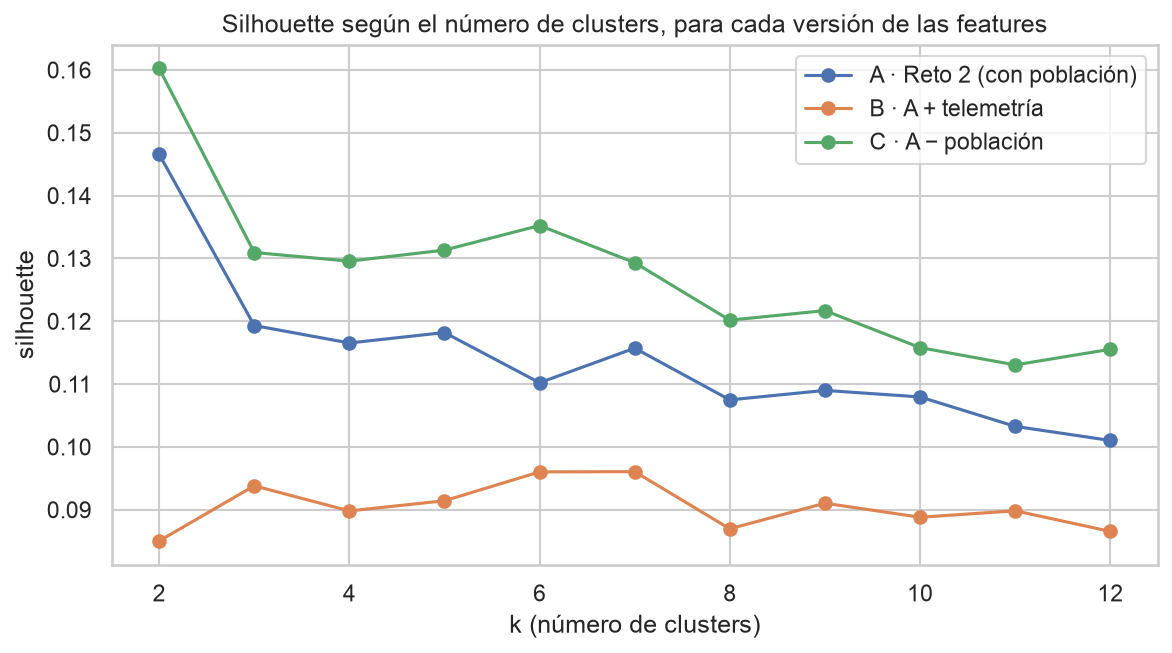
\includegraphics[width=0.62\linewidth]{03_silhouette_versiones.png}
\caption{Silhouette por $k$: A (variables del reto 2), B (A + telemetría) y C (A sin población).}
\end{figure}

La telemetría empeora el modelo \textbf{en los 11 valores de $k$}: rellenar con la mediana al 40\,\% que no la tiene los apila a todos en el mismo punto. Quitar la población lo mejora también en los 11, porque casi no se relaciona con nada y solo añade dispersión. Nos quedamos con la versión C. Antes de agrupar comprobamos además que ninguna pareja de variables distintas supera una correlación de 0,7 (la máxima es 0,63). El único valor alto ($-0{,}86$) está entre dos columnas \textit{one-hot} de la misma variable, y es así por construcción.

\subsection*{Eligiendo $k$}

\begin{figure}[H]
\centering
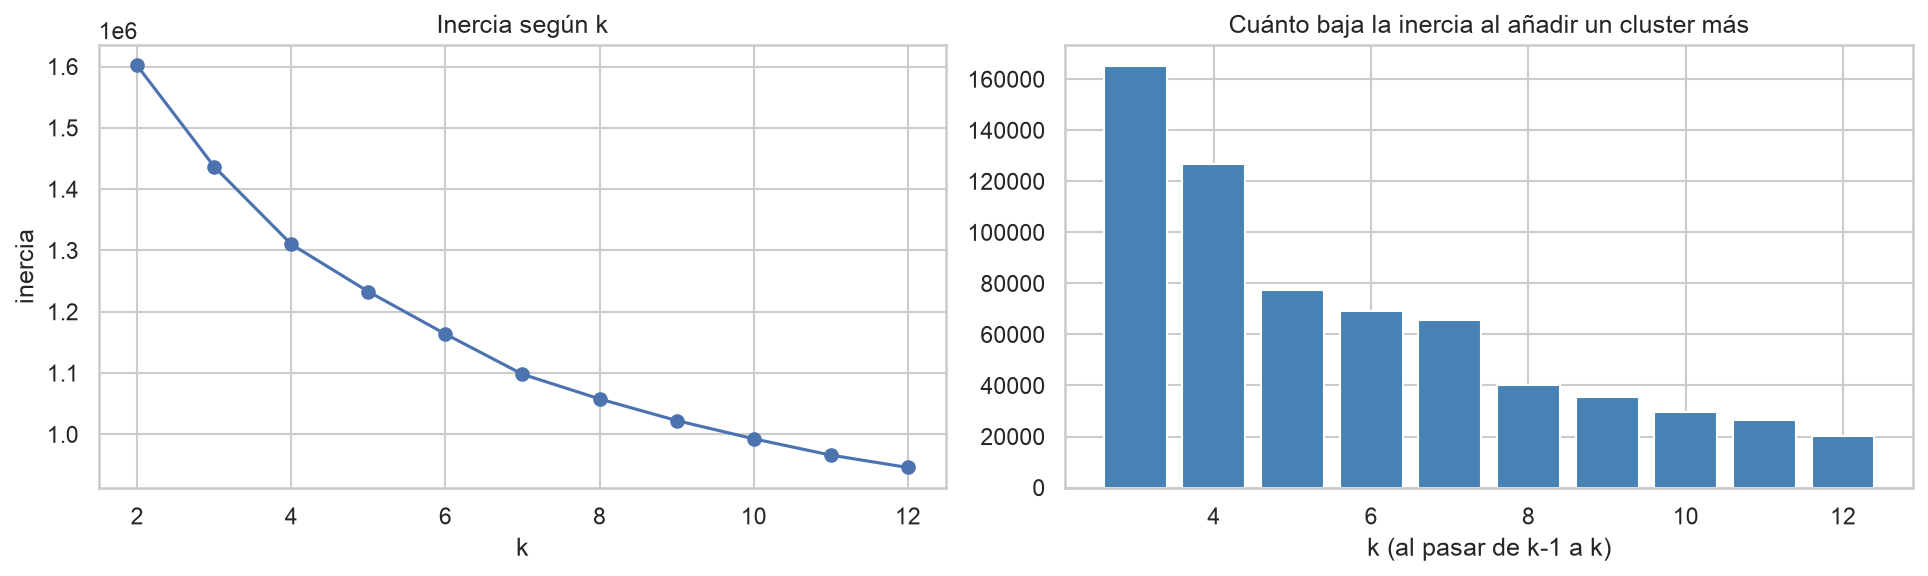
\includegraphics[width=\linewidth]{03_codo.png}
\caption{Método del codo: inercia y cuánto baja al añadir cada cluster.}
\end{figure}

Miramos cinco criterios a la vez, porque ninguno basta solo:

\begin{itemize}
  \item \textbf{Codo.} La curva no tiene un codo nítido, pero la mejora al añadir clusters muestra dos escalones. Pasar de 3 a 4 quita 126.000 de inercia y de 4 a 5, 77.000. Entre 5 y 7 la mejora se mantiene (69.000 y 66.000), y de 7 a 8 cae a 40.000. El último escalón está en $k=7$.
  \item \textbf{Silhouette.} Es bajo en todos los $k$ (de 0,11 a 0,16), cosa esperable con datos de clientes reales y muchas variables binarias. Se mantiene plano entre 3 y 7 (alrededor de 0,13), con un pico en $k=6$ (0,135), y baja a partir de 8. Lo usamos para comparar, no como nota.
  \item \textbf{Davies-Bouldin.} Mejora hasta $k=7$--8 (1,82 en $k=7$).
  \item \textbf{Tamaño mínimo.} Con $k=7$, el cluster más pequeño tiene el 5,6\,\% de los clientes; ninguno es residual.
  \item \textbf{Estabilidad.} Entrenamos cada $k$ con cuatro semillas y comparamos con el ARI. \textbf{$k=6$ es inestable} (ARI de 0,54 con dos de las semillas): su pico de silhouette depende del azar. $k=7$ sale prácticamente idéntico con todas (1,00, 1,00 y 0,99).
\end{itemize}

Nos quedamos con \textbf{$k=7$}. Coincide con el último escalón del codo, está entre los mejores en silhouette y Davies-Bouldin, es estable y siete segmentos son manejables para un equipo de marketing. Los clusters quedan numerados por tamaño, del 24,1\,\% al 5,6\,\%. Por cluster, el más nítido es el de los electrificados (silhouette 0,16) y el más difuso el de multivehículo (0,07), que mezcla familias con varios coches y flotas.

\section{Reto 4 · Interpretación de los segmentos}

\subsection*{Cómo perfilamos}

Cada segmento lo comparamos siempre con el total de clientes, midiendo cuántas desviaciones típicas se separa de la media en cada indicador. Que un segmento tenga 48 meses de antigüedad no dice nada; que los tenga cuando la media es 34, sí. Todas las cifras salen de un mismo módulo (\var{src/profiling.py}), y los textos de cada segmento no llevan números escritos a mano: llevan huecos que se rellenan con el dato, para que no pueda haber incoherencias.

\begin{figure}[H]
\centering
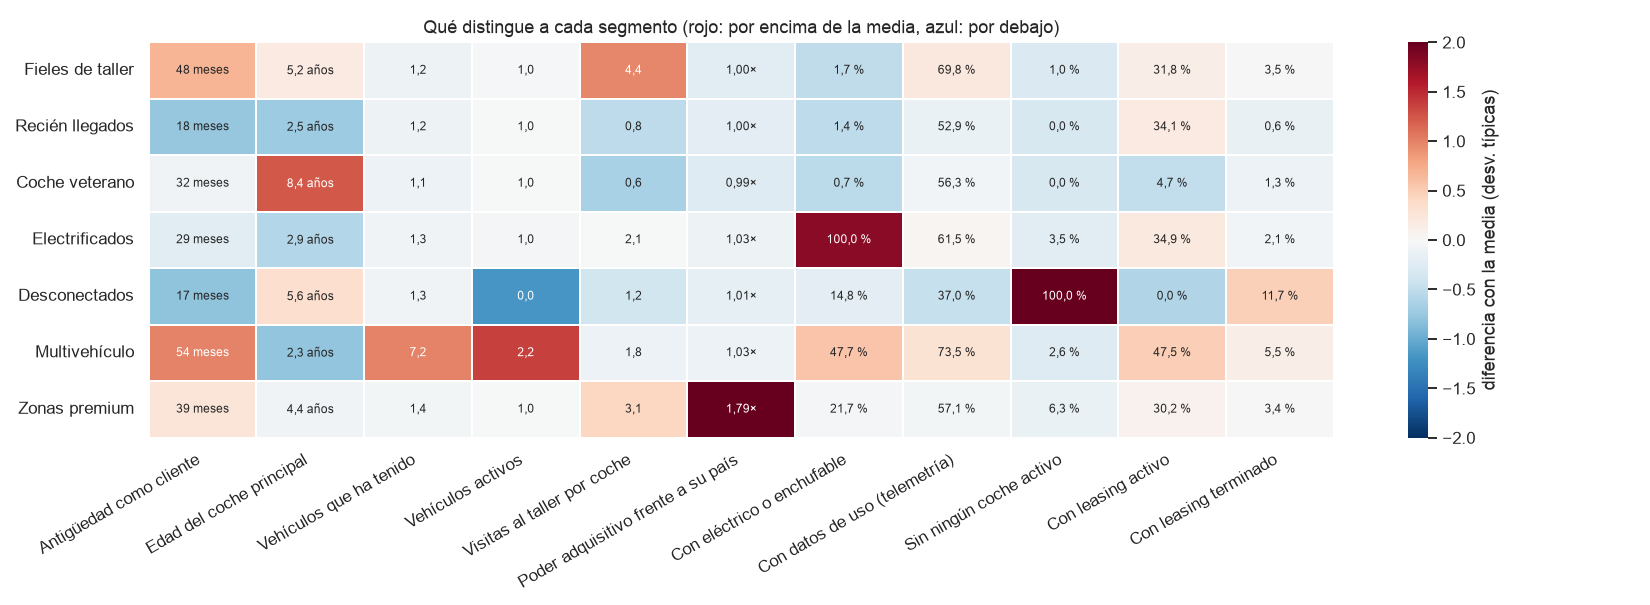
\includegraphics[width=\linewidth]{04_mapa_calor.png}
\caption{Qué distingue a cada segmento. Rojo: por encima de la media; azul: por debajo. En cada casilla, el valor real.}
\end{figure}

\subsection*{Los siete segmentos}

\begin{table}[H]
\centering\small
\begin{tabularx}{\linewidth}{>{\raggedright\arraybackslash}p{2.6cm}r>{\raggedright\arraybackslash}p{5.4cm}L}
\toprule
Segmento & \% & Lo que le define & Qué hacemos \\
\midrule
\textbf{Coche en garantía} & 24,1 & El que más ha usado la garantía (4,4 visitas por coche, frente a 2,1), 48 meses con la marca y coche de unos 5 años & \textbf{Retener}: extensión de garantía o contrato de mantenimiento antes de que venza \\
\textbf{Recién llegados} & 18,3 & 18 meses como clientes y coche de 2,5 años & \textbf{Vincular}: primera revisión en el taller oficial y bienvenida; aún no toca cambiar de coche \\
\textbf{Coche veterano} & 18,2 & Coche de 8,4 años, casi sin leasing (4,7\,\%) y más de la mitad sin visitas en garantía & \textbf{Renovar}: valoración de su coche y financiación; traerlo al taller oficial \\
\textbf{Electrificados} & 15,9 & Todos con eléctrico o enchufable (la media es 23\,\%), coche reciente & \textbf{Acompañar}: siguiente eléctrico, servicios de carga y \textit{wallbox} \\
\textbf{Desconectados} & 9,0 & Ningún coche activo y 11,7\,\% con leasing terminado (la media es 3,3\,\%) & \textbf{Recuperar}: oferta de vuelta y averiguar quién se ha ido de verdad \\
\textbf{Multivehículo} & 8,8 & 7,2 vehículos de media y 54 meses con la marca; aquí están 904 de las 908 cuentas grandes & \textbf{Ampliar}: gestor de cuenta y renovación de flota \\
\textbf{Zonas premium} & 5,6 & Zona con 1,79 veces el poder adquisitivo típico de su país, casi todos en Suiza & \textbf{Elevar}: gama alta y servicio premium \\
\bottomrule
\end{tabularx}
\end{table}

Para los nombres seguimos cuatro reglas: dos o tres palabras, que describan el comportamiento y no la demografía, que se entiendan sin saber qué es K-Means y que no juzguen al cliente. Por eso ``Desconectados'' y no ``Perdidos'': no tener coche activo no prueba que se hayan ido.

\subsection*{Tres cosas que aprendimos al interpretar}

\begin{itemize}
  \item \textbf{No hay un segmento de furgonetas.} Las furgonetas se concentran algo en Recién llegados y Multivehículo (alrededor del 20\,\%, frente al 11\,\% del total), pero en ningún segmento son mayoría. Es consecuencia de dejar las \textit{one-hot} en 0/1: los segmentos los definen la relación con la marca y el ciclo de vida del coche, no el producto. Nos parece más útil, porque dice \emph{cuándo} y \emph{cómo} hablar a cada cliente; el producto se ajusta dentro de cada segmento.
  \item \textbf{Las visitas al taller son solo visitas en garantía.} Suben con la edad del coche hasta los 5--6 años y luego bajan. Por eso el segmento con más visitas tiene el coche en esa edad, y el de coche veterano apenas tiene ninguna. No miden fidelidad al taller, sino uso de la garantía. Lo tuvimos en cuenta al elegir los nombres y las acciones.
  \item \textbf{Los canales de contacto son iguales en todos los segmentos} (email 98\,\%, teléfono 86\,\%, correo 85\,\%). El canal se elige por el mensaje, no por el segmento.
\end{itemize}

Todo esto está también en un \textbf{dashboard} (\var{outputs/dashboard\_segmentos.html}). Es un único fichero que se abre en cualquier navegador sin instalar nada y que solo lleva datos agregados. Tiene una vista general y una ficha por segmento con su plan en las cuatro palancas del reto: oferta de vehículo, mantenimiento, fidelización y comunicación.

\section{Resultado final}

Partimos de 302.850 filas cliente-vehículo y terminamos con \textbf{siete segmentos de clientes estables}, cada uno con un rasgo claro y una acción concreta: retener, vincular, renovar, acompañar, recuperar, ampliar y elevar. Por el camino:

\begin{itemize}
  \item Pasamos el análisis a nivel cliente, que era la decisión que más cambiaba los resultados.
  \item Arreglamos lo que se podía arreglar (el motor por versión comercial, el valor por defecto de la antigüedad) y no rellenamos lo que habría sido inventar (la telemetría, el género).
  \item Elegimos cada variable y cada parámetro con un dato delante. Cuando una idea no aportaba, como la población o la telemetría, la quitamos.
  \item Elegimos $k$ mirando también la estabilidad, que fue lo que descartó $k=6$.
\end{itemize}

Hay límites que conviene tener presentes. El silhouette es bajo (0,13), algo normal con datos mixtos de clientes reales: los segmentos son zonas con más densidad, no grupos aislados. ``Sin coche activo'' es una señal de fuga, no una prueba. Y en el 12\,\% de los clientes la antigüedad es un valor por defecto. En los retos avanzados compararemos K-Means con otros algoritmos, veremos los segmentos en dos dimensiones con PCA y mediremos su estabilidad con Jackknife.

\end{document}
